\subsection{Standard Model QCD Multijet and all Hadronic $\ttbar$}
\label{sec:Bkg:QCD}

\indent Both QCD multijet and all hadronic $\ttbar$ creates little intrinsic $\met$. Instead misreconstructed jets can cause an imbalance in the total event $E_t$ and generate fake $\met$.  QCD contributions are only significant in the SR bins with low $\RISR < 0.4$ and are estimated using the data driven jet smearing method.  \\

\subsubsection*{The Jet Smearing Method}

\indent The jet smearing method first selects seed events from data with well reconstructed jets and little $\met$.  Seed events are selected according to the criteria listed in table \ref{tab:qcd:seed}. We then repeatedly smear the seed events' jets with a predetermined jet energy response.  The resulting {\tt pesudo-data} events can have potentially large $\met$ due to the smeared jets.  A schematic demonstrating the jet smearing method is shown in figure \ref{fig:jetsmearing}.\\

\begin{figure}[htbp]
\begin{center}
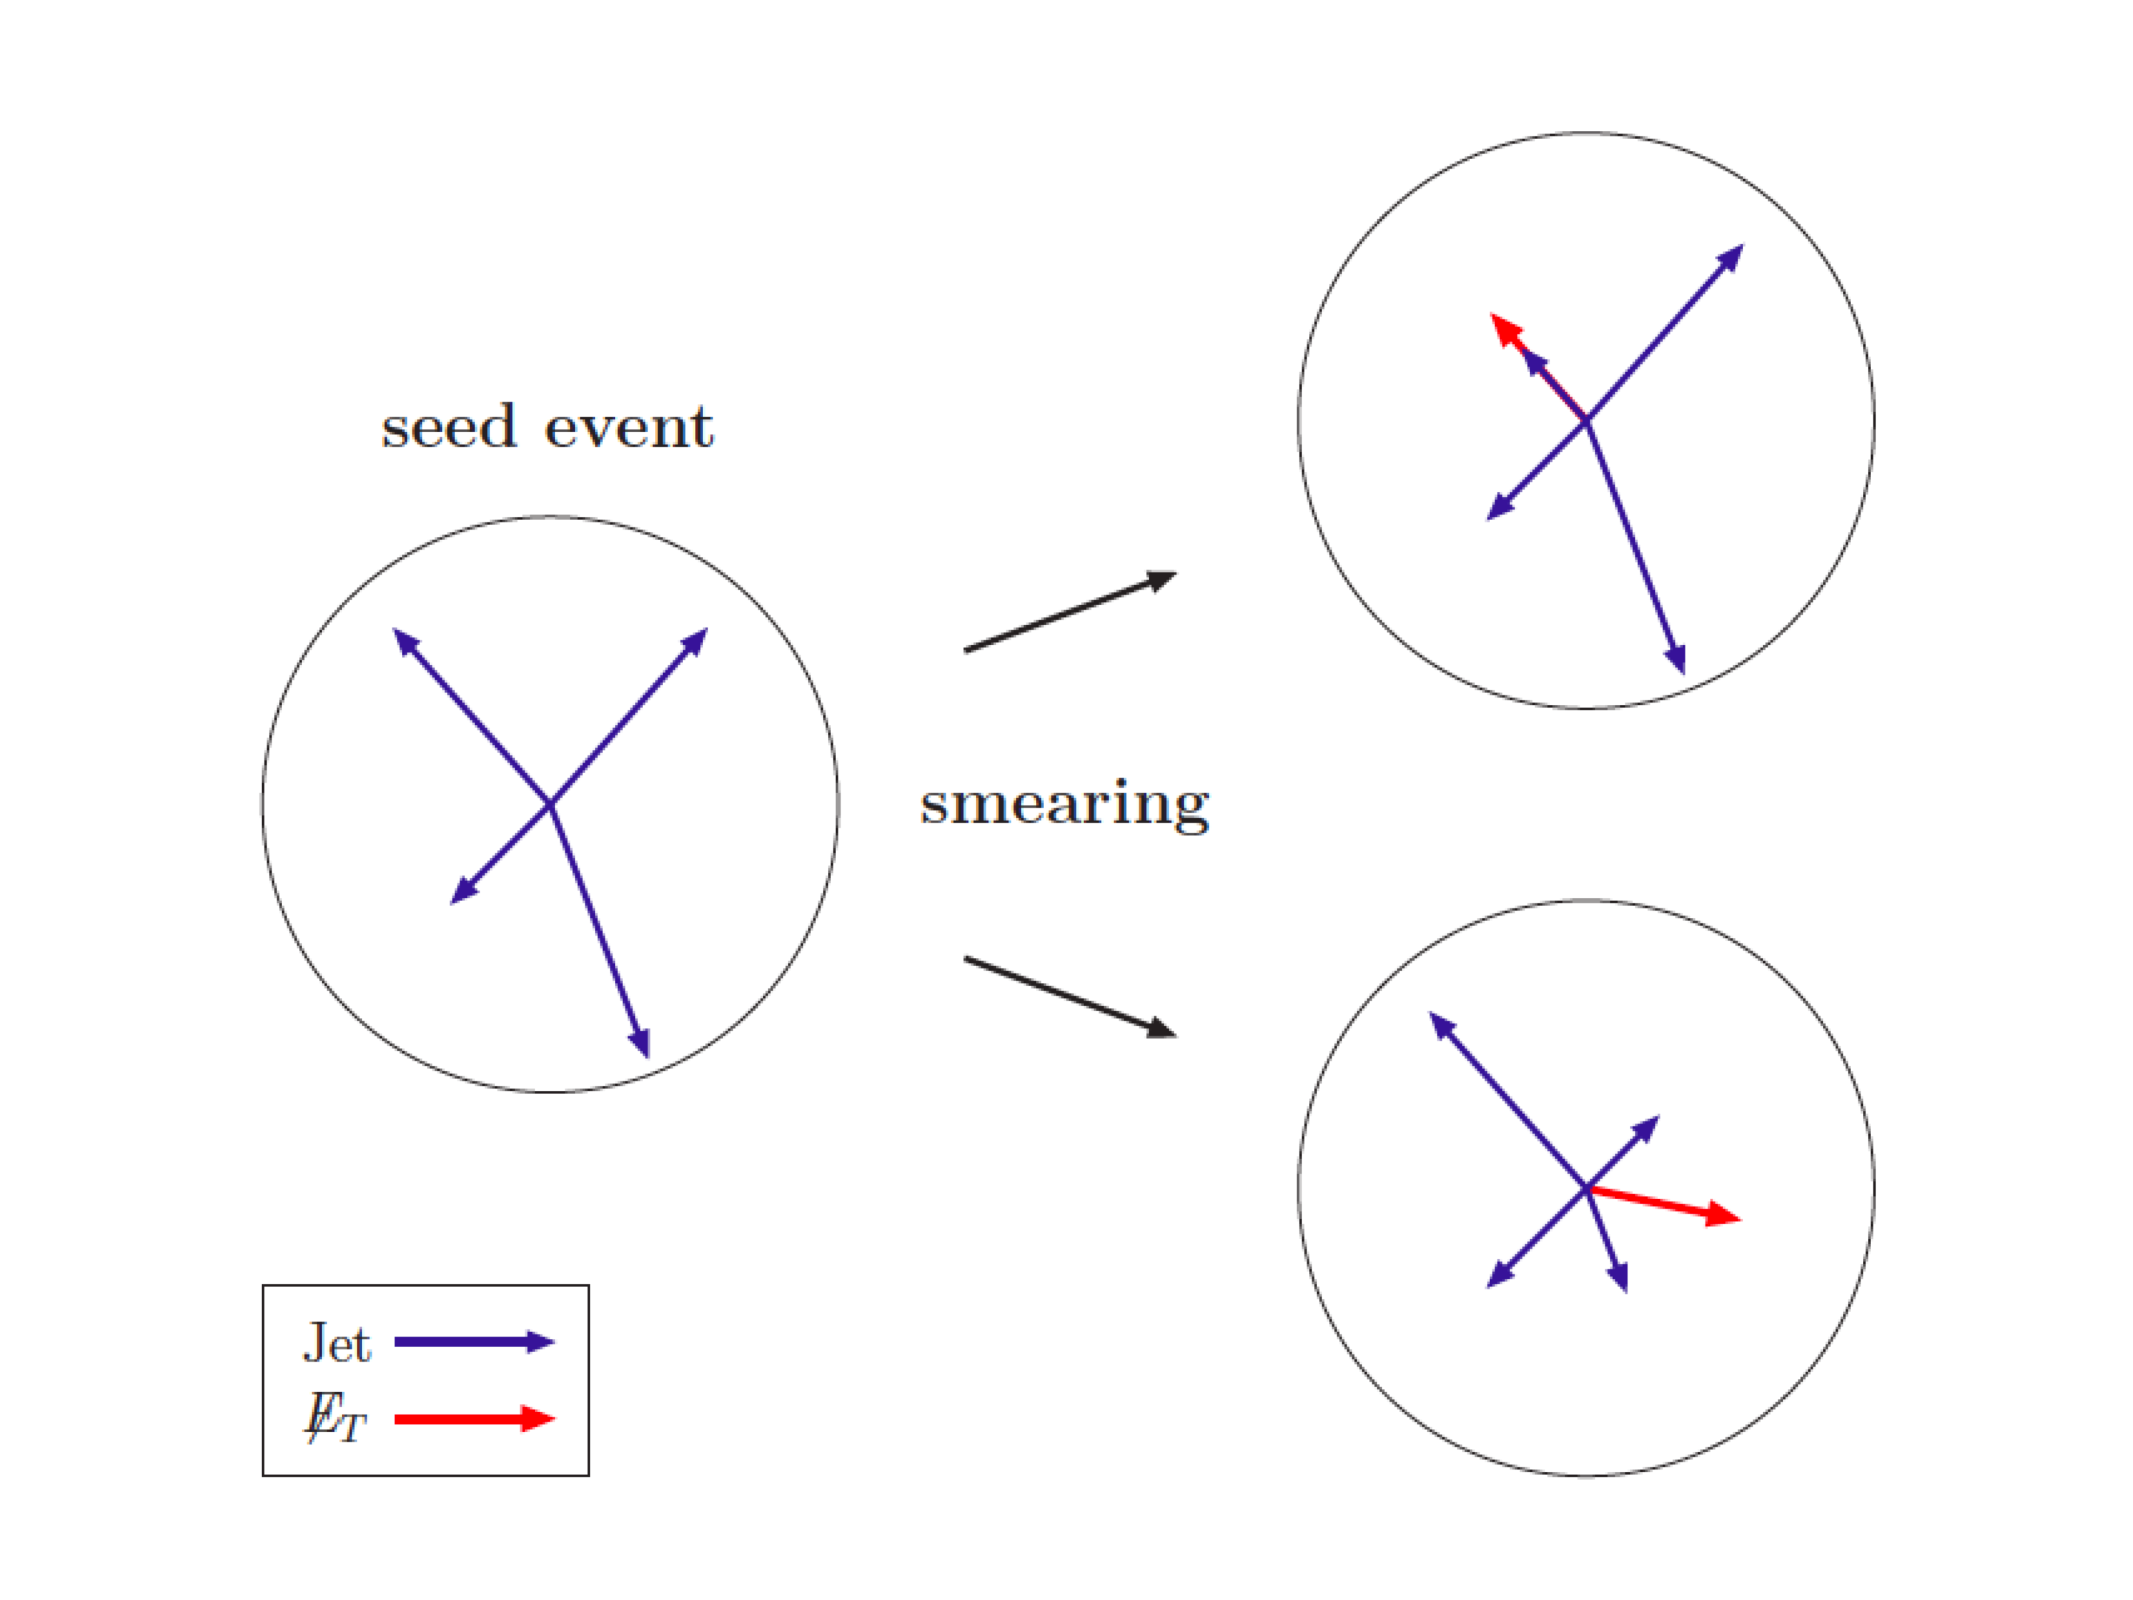
\includegraphics[width=0.45\textwidth]{figures/QCDJetSmearing/jet_smearing.pdf}
\end{center}
\caption{Schematic of the jet smearing method.  A seed event with good jet energy measurements are repeatedly smeared with predetermined jet energy resolutions.  The new $\met$ is calculated as the difference between the seed event's and smeared event's jet momenta plus the original seed event's $\met$.  (Figure taken from \cite{JetSmearing})}
\label{fig:jetsmearing}
\end{figure}

\indent The jet smearing methods have a number of inherent assumptions about the generation of $\met$ in QCD multijet and all hadronic $\ttbar$ background.  These assumptions include: \\

\begin{itemize}
\item The jet response captures all sources of jet $\pt$ measurement fluctuations
\item The $\met$ in multijet events result predominately from mis-measured jets
\item Jet response are independent on the presence of other jet and jet smearing can be applied on a jet-by-jet basis
\end{itemize}

\indent These assumptions seem be well satisfied in the high $\met$, high jet multiplicity region of SR.   We also validate QCD predictions in a QCD VR defined in section \ref{sec:QCD:CR}.\\

\indent Other sources of $\met$ not taken into account by the jet smearing method such as $\met$ from pileup jets, mis-reconstructed soft term of the $\met$ and object overlap removal are assumed to be negligible in the SR. \\

 \begin{table}[htp]
 \caption{Seed event preselection}
 \begin{center}
 \begin{tabular}{c} \hline
   Cut\\ \hline
   $n_\mathrm{prim. vertices} > 0$\\
   Jet trigger\\
   Bad jet veto\\
   Cosmic muon veto\\
   Bad muon veto\\
   {\tt Baseline} lepton veto\\
   $\geq 4$ jets\\
   $\geq 1$ $b$-jets\\
   $\met\rm{sig.} < 0.3 + 0.1\cdot n_{\textup{n-bjets}}$ \\ \hline
 \end{tabular}
 \end{center}
 \label{tb:seed_events_presel}
 \end{table}

\indent The quantity $\met\rm{sig.}=\frac{ \met-8\rm{\,GeV} } {\sum E_\mathrm{T} }$ measures the general significance of $\met$ relative to total hadronic activity in an event.  In general events with low $\met\rm{sig.}$ have better reconstructed jets.  However, the requirement on $\met\rm{sig.}$ depends on the number of b-jets because b-quarks can emit significant portions of their energy in the form of neutrinos.  \\

\indent The jet response function include contributions from the following effects: \\

\begin{itemize}
\item Limited calorimeter granularity
\item Hadronic energy falling outside of the jet radius or failed to be clustered correctly by jet reconstruction.
\item Additional energy clustered into the jet that result from other sources.
\item Energetic jet punching through the calorimeter.
\item Dead material in the calorimeter.
\item b-quark generating real $\met$ through decay to neutrinos.  B-tagged jets have a different jet response function than light quark jets to account for this difference.
\end{itemize}

\subsubsection*{QCD multijet Control Region and Validation Region}
\label{sec:QCD:CR}

\indent The pseudo-data resulting from the jet smearing processes is then normalized to data using the QCD control region defined in table \ref{tab:QCDCR}.  The QCD CR is designed to be similar to the SR except the $\mindphijettwomet$ is required to be between $0.05$ to $0.1$ instead of greater than $0.04$.  This region is dominated by QCD backgrounds with high $\met$ due to a single mis-reconstructed energetic jet but with the same jet multiplicity and jet kinematics required in the SR. \\

\begin{table}[htpb]
  \begin{center}
    \def\arraystretch{1.4}%
    \begin{tabular}{c|c} \hline\hline
      {\bf Variable} &  CR  \\ \hline \hline
      \mindphijettwomet  & [0.05,0.1]  \\  
      \nBJetS & {$\ge1$} \\
      \nJetS & {$\ge5$}  \\
      \pTSBZero &{$>40\gev$}  \\
      \dPhiISRMET &  $>2.00$  \\ 
      \pTISR & $>150$ GeV   \\
      \rISR  & {$<0.4$} \\
      \pTSFour & {$>50$ GeV}   \\ \hline
       b-tagged jets &{$\ge1$} \\ \hline \hline
    \end{tabular}
  \caption{QCD CR definitions, in addition to the zero lepton preselection in Table~\ref{tab:0Lcommon}. }
     \label{tab:QCDCR}
  \end{center}
\end{table}%

\indent Data vs QCD pseudo-data prediction for the $\PTISR$, $\dphiISRI$ and $\MS$ variables for the QCD CR can be seen in figure \ref{fig:QCD:CR}.  These variables are shown because they are extrapolated over from CR to SR. \\

\begin{figure}[!htbp]
\begin{center}
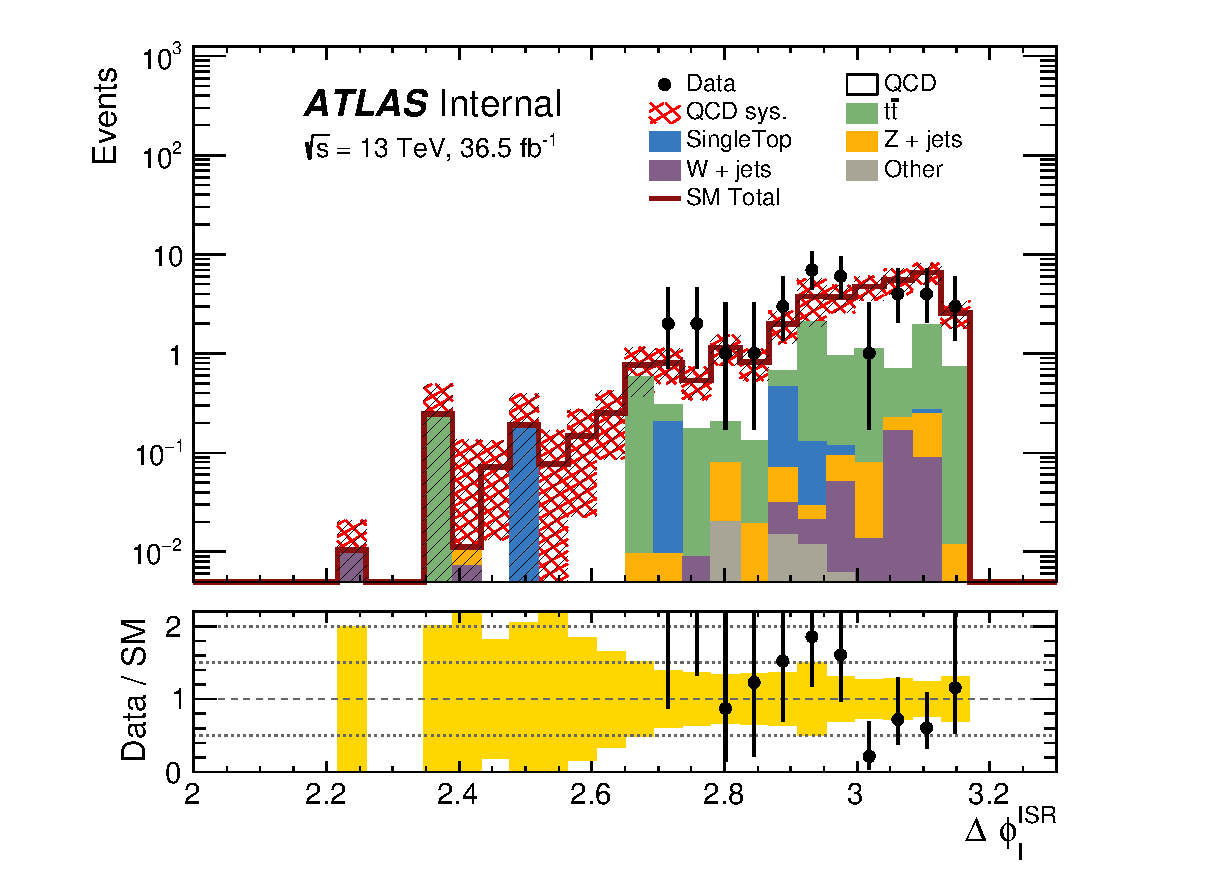
\includegraphics[width=0.48\textwidth]{figures/QCDJetSmearing/CRQC/dphiISRI_36500.eps}
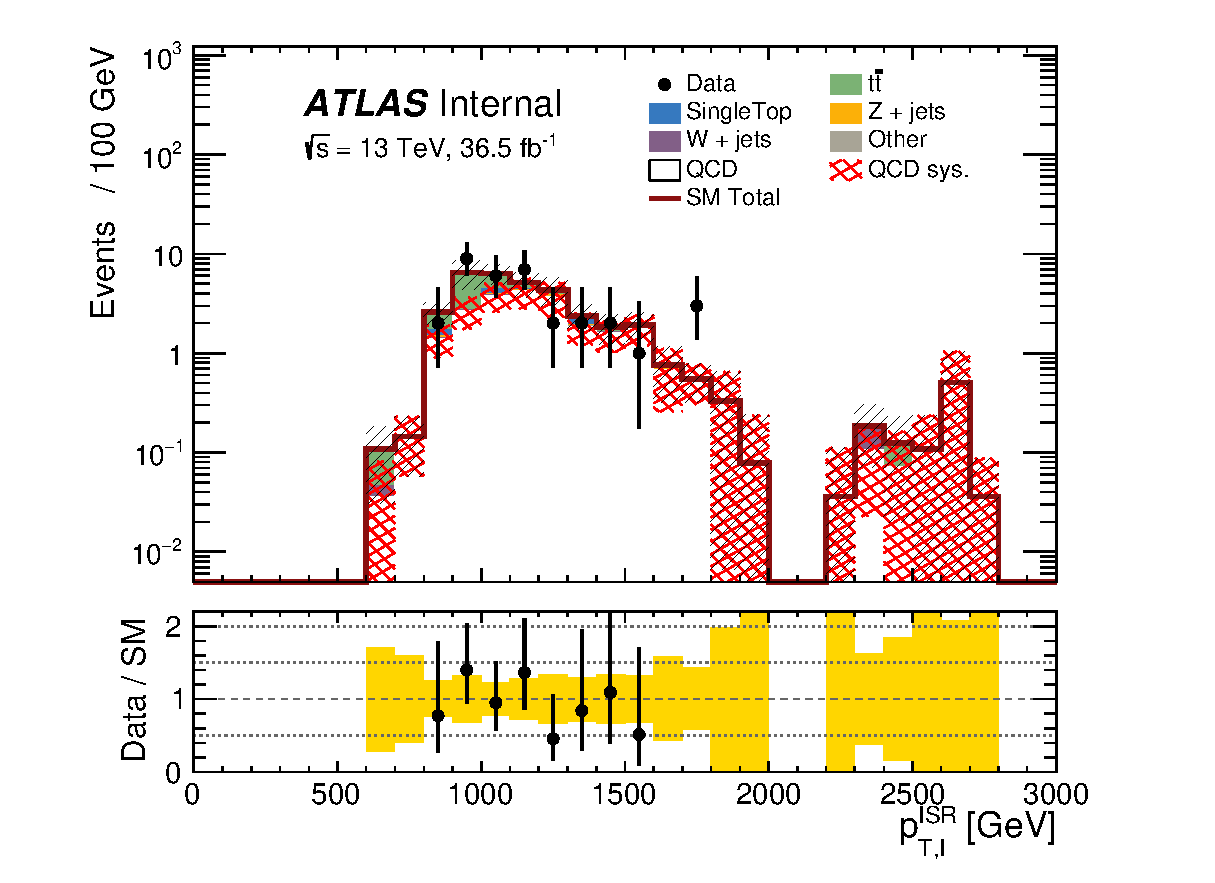
\includegraphics[width=0.48\textwidth]{figures/QCDJetSmearing/CRQC/PTISR_36500}
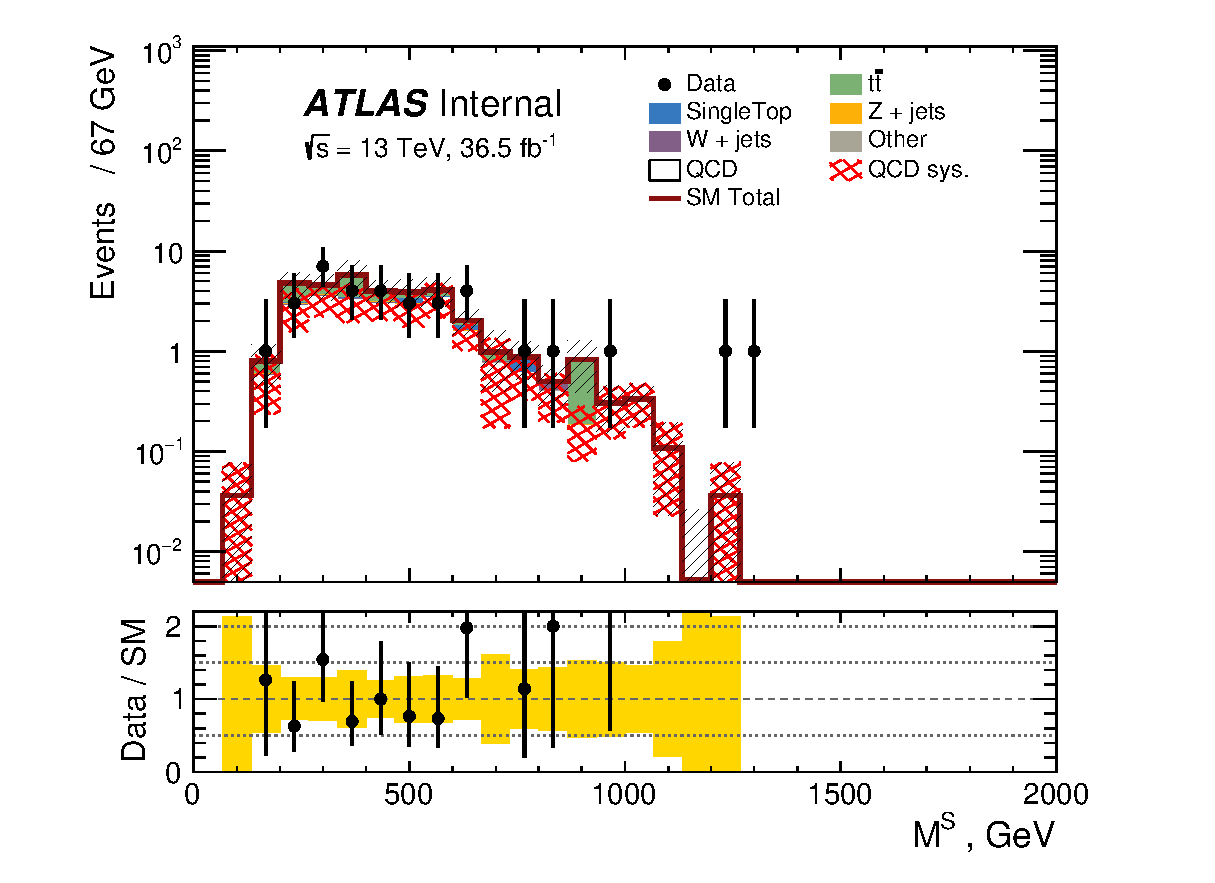
\includegraphics[width=0.48\textwidth]{figures/QCDJetSmearing/CRQC/MV_36500}
\caption{$\PTISR$, $\dphiISRI$ and $\MS$ distributions in the QCD control regions.}
\label{fig:QCD:CR}
\end{center}
\end{figure}

\indent The results of QCD multijet prediction using jet smearing after normalizing to the CR can be checked in the QCD VR defined in table \ref{tab:QCDVR}.   The QCD VR has the exact same kinematic selection as the SR except with a lower $\mindphijettwomet$ between $0.1$ and $0.2$.  $\RISR$ is also required to be below $0.4$ as we don't expect significant QCD contribution at higher $\RISR$.  \\

\begin{table}[htpb]
  \caption{QCD VR definitions, in addition to the 0 lepton preselection in Table~\ref{tab:0Lcommon}. }
   \label{tab:QCDVR}
  \begin{center}
    \def\arraystretch{1.4}%
    \begin{tabular}{c|c} \hline\hline
      {\bf Variable} &  VR  \\ \hline \hline
      \mindphijettwomet  &  [0.1,0.2]           \\  
      \nBJetS & $\ge1$ \\
      \nJetS & $\ge5$  \\
      \pTSBZero & $>40\gev$  \\ 
      \mS & $>300\gev$  \\
      \dPhiISRMET &  $>3.00$  \\ 
      \pTISR & $>400$ GeV \\ 
      \rISR  & $<0.4$ \\
      \pTSFour & $>50$ GeV  \\ \hline
       b-tagged jets & $\ge1$  \\ \hline \hline
    \end{tabular}
  \end{center}
\end{table}%

\indent Data vs QCD pseudo-data prediction for the $\RISR$ and $\dphiISRI$ variables for the QCD VR can be seen in figure \ref{fig:QCD:CR}.  A good agreement is found between data and pseudo-data predictions. \\

\begin{figure}[!htbp]
\begin{center}
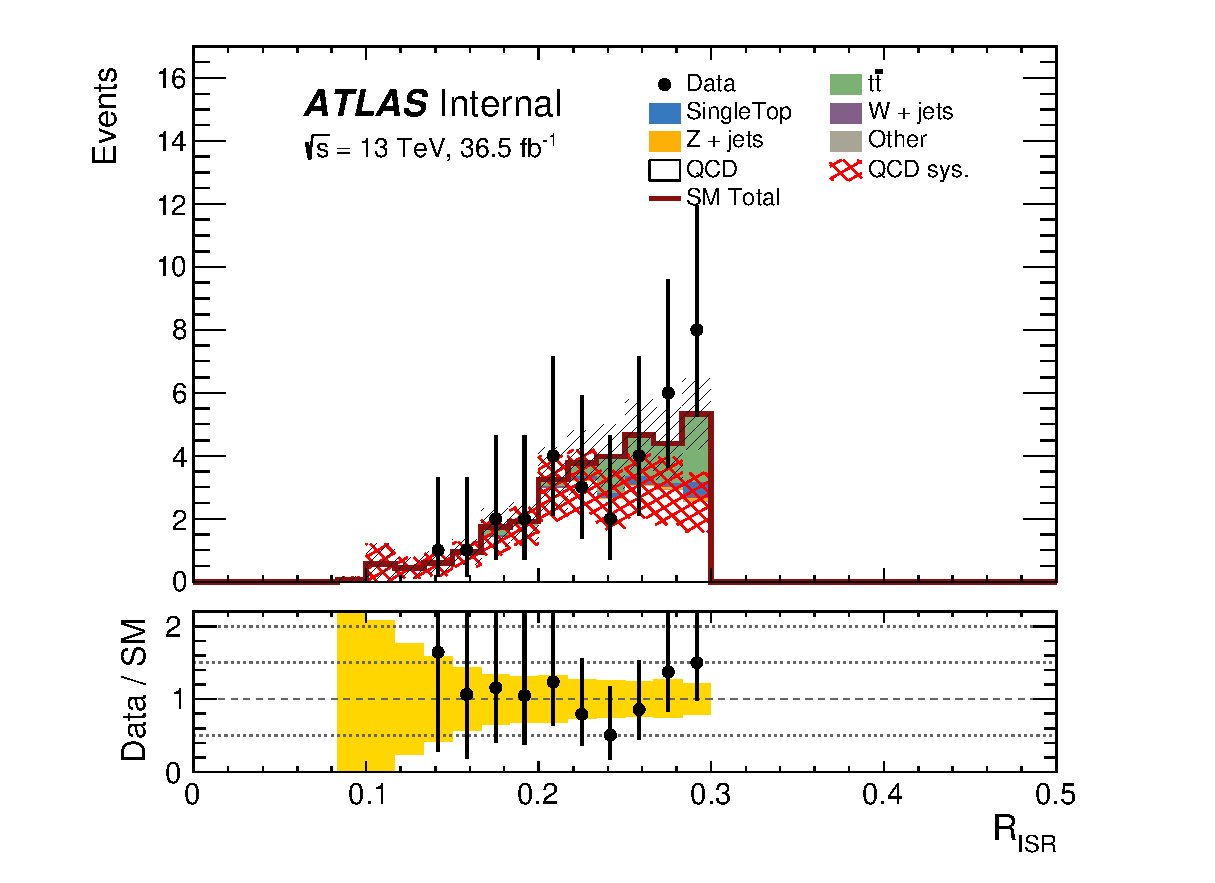
\includegraphics[width=0.48\textwidth]{figures/QCDJetSmearing/VRqC/RISR_36500} 
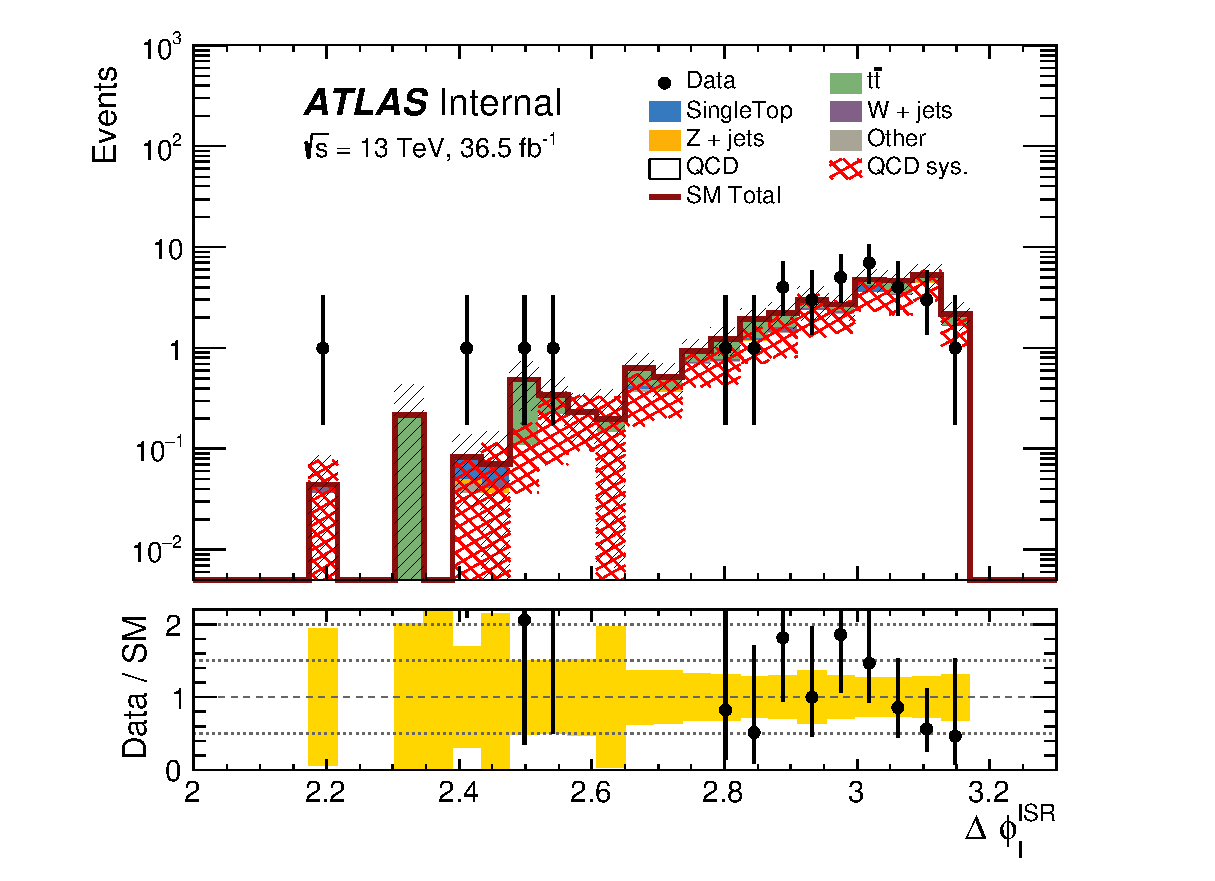
\includegraphics[width=0.48\textwidth]{figures/QCDJetSmearing/VRqC/dphiISRI_36500.eps}
\caption{$\RISR$ and $\dphiISRI$ distributions in the QCD validation regions.}
\label{fig:QCD:VR}
\end{center}
\end{figure}

\subsubsection*{QCD prediction in the Signal Region}

\indent The predicted amount of QCD in the SR is given by the amount of QCD pseudo-data that survive the SR selection after normalization to the QCD CR. The systematic uncertainty on the SR QCD prediction is given by repeating the process with a tighter and looser set of seed event selections.  An upward error correspond to seed events requiring $\met\rm{sig.} < 0.6 + 0.2\cdot n_{\textup{n-bjets}}$ and an lower error corresponds to seed events requiring $\met\rm{sig.} < 0.2 + 0.05\cdot n_{\textup{n-bjets}}$. \\

\indent The expected QCD yield and uncertainty in the SR is given in table \ref{tab:QCD:SRyield}

\begin{table}[!htbp]
  \begin{center}
    \begin{tabular}{c|c|c|c|c|c} \hline\hline
SR $\RISR$ Region       & 0.3-0.4              & 0.4-0.5              & 0.5-0.6              & 0.6-0.7             & 0.7-0.8 \\ \hline
QCD expected yield & $4.56\pm2.38$ & $1.58\pm0.77$ & $0.32\pm0.17$ & $0.04\pm0.02$ & $0.00\pm0.00$ \\ \hline \hline
    \end{tabular}
  \caption{Expected yields of the QCD multijet backgrounds in SR.}
  \label{tab:QCDYields}
  \end{center}
\end{table}%
